%===============================================================================
% LaTeX sjabloon voor de bachelorproef toegepaste informatica aan HOGENT
% Meer info op https://github.com/HoGentTIN/bachproef-latex-sjabloon
%===============================================================================

\documentclass[dvipsnames]{bachproef-tin}

\usepackage{hogent-thesis-titlepage} % Titelpagina conform aan HOGENT huisstijl
\usepackage{tabularx}
\usepackage{xcolor}
\usepackage{listings}

\renewcommand\lstlistlistingname{Codevoorbeeld}
\renewcommand{\lstlistingname}{Codevoorbeeld}

\lstdefinestyle{mystyle}{
	basicstyle=\ttfamily\footnotesize,
	breakatwhitespace=false,         
	breaklines=true,                 
	captionpos=b,                    
	keepspaces=true,                 
	numbers=left,                    
	numbersep=5pt,                  
	showspaces=false,                
	showstringspaces=false,
	showtabs=false,                  
	tabsize=2
}

\lstset{
	basicstyle=\scriptsize\sffamily\color{black},
	frame=single,
	numbers=left,
	numbersep=5pt,
	numberstyle=\tiny\color{gray},
	tabsize=1
}
\lstset{style=mystyle}

\lstdefinelanguage{Kotlin}{
	comment=[l]{//},
	commentstyle={\color{gray}\ttfamily},
	emph={delegate, filter, first, firstOrNull, forEach, lazy, map, mapNotNull, println, return@},
	emphstyle={\color{OrangeRed}},
	identifierstyle=\color{black},
	keywords={abstract, actual, as, as?, break, by, class, companion, continue, data, do, dynamic, else, enum, expect, false, final, for, fun, get, if, import, in, interface, internal, is, null, object, override, package, private, public, return, set, super, suspend, this, throw, true, try, typealias, val, var, vararg, when, where, while},
	keywordstyle={\color{NavyBlue}\bfseries},
	morecomment=[s]{/*}{*/},
	morestring=[b]",
	morestring=[s]{"""*}{*"""},
	ndkeywords={@Deprecated, @JvmField, @JvmName, @JvmOverloads, @JvmStatic, @JvmSynthetic, Array, Byte, Double, Float, Int, Integer, Iterable, Long, Runnable, Short, String},
	ndkeywordstyle={\color{BurntOrange}\bfseries},
	sensitive=true,
	stringstyle={\color{ForestGreen}\ttfamily},
}

\lstdefinelanguage{JavaScript}{
	keywords={typeof, new, true, false, catch, function, return, null, catch, switch, var, if, in, while, do, else, case, break},
	keywordstyle=\color{blue}\bfseries,
	ndkeywords={class, export, boolean, throw, implements, import, this},
	ndkeywordstyle=\color{darkgray}\bfseries,
	identifierstyle=\color{black},
	sensitive=false,
	comment=[l]{//},
	morecomment=[s]{/*}{*/},
	commentstyle=\color{purple}\ttfamily,
	stringstyle=\color{red}\ttfamily,
	morestring=[b]',
	morestring=[b]"
}



%%---------- Documenteigenschappen ---------------------------------------------
% TODO: Vul dit aan met je eigen info:
% https://tex.stackexchange.com/questions/60209/how-to-add-an-extra-level-of-sections-with-headings-below-subsubsection
% De titel van het rapport/bachelorproef
\title{Progressive web application vs Native application}

% Je eigen naam
\author{Robbie Verdurme}

% De naam van je promotor (lector van de opleiding)
\promotor{Lieven Smits}

% De naam van je co-promotor. Als je promotor ook je opdrachtgever is en je
% dus ook inhoudelijk begeleidt (en enkel dan!), mag je dit leeg laten.
\copromotor{Bart Delrue}

% Indien je bachelorproef in opdracht van/in samenwerking met een bedrijf of
% externe organisatie geschreven is, geef je hier de naam. Zoniet laat je dit
% zoals het is.
\instelling{Digipolis}

% Academiejaar
\academiejaar{2018-2019}

% Examenperiode
%  - 1e semester = 1e examenperiode => 1
%  - 2e semester = 2e examenperiode => 2
%  - tweede zit  = 3e examenperiode => 3
\examenperiode{2}

%===============================================================================
% Inhoud document
%===============================================================================

\begin{document}

%---------- Taalselectie -------------------------------------------------------
% Als je je bachelorproef in het Engels schrijft, haal dan onderstaande regel
% uit commentaar. Let op: de tekst op de voorkaft blijft in het Nederlands, en
% dat is ook de bedoeling!

%\selectlanguage{english}

%---------- Titelblad ----------------------------------------------------------
\inserttitlepage

%---------- Samenvatting, voorwoord --------------------------------------------
\usechapterimagefalse
%%=============================================================================
%% Voorwoord
%%=============================================================================

\chapter*{\IfLanguageName{dutch}{Woord vooraf}{Preface}}
\label{ch:voorwoord}

%% TODO:
%% Het voorwoord is het enige deel van de bachelorproef waar je vanuit je
%% eigen standpunt (``ik-vorm'') mag schrijven. Je kan hier bv. motiveren
%% waarom jij het onderwerp wil bespreken.
%% Vergeet ook niet te bedanken wie je geholpen/gesteund/... heeft
In deze bachelorproef wordt er een vergelijking gemaakt tussen een native applicatie en een progressive web applicatie. De reden hiervoor is mijn stageplaats bij Digipolis. Digipolis wil graag onderzoeken wat de mogelijkheden van een progressive web applicatie zijn, zodat deze technologie eventueel gebruikt kan worden binnen het bedrijf. De reden waarom digipolis dit wilt onderzoeken is om te weten te komen of applicaties een meerwaarde kunnen bieden voor de doelstellingen van digipolis (burgers informeren en helpen participeren) en welke methode best past binnen hun ecosysteem.

Graag wil ik mijn promotor Lieven Smits bedanken voor de feedback en de steun tijdens het schrijven van de bachelorproef. Daarnaast wil ik ook Bart Delrue bedanken voor de technische feedback en de begeleiding tijdens het verloop van de bachelorproef.




%%=============================================================================
%% Samenvatting
%%=============================================================================

% TODO: De "abstract" of samenvatting is een kernachtige (~ 1 blz. voor een
% thesis) synthese van het document.
%
% Deze aspecten moeten zeker aan bod komen:
% - Context: waarom is dit werk belangrijk?
% - Nood: waarom moest dit onderzocht worden?
% - Taak: wat heb je precies gedaan?
% - Object: wat staat in dit document geschreven?
% - Resultaat: wat was het resultaat?
% - Conclusie: wat is/zijn de belangrijkste conclusie(s)?
% - Perspectief: blijven er nog vragen open die in de toekomst nog kunnen
%    onderzocht worden? Wat is een mogelijk vervolg voor jouw onderzoek?
%
% LET OP! Een samenvatting is GEEN voorwoord!

%%---------- Nederlandse samenvatting -----------------------------------------
%
% TODO: Als je je bachelorproef in het Engels schrijft, moet je eerst een
% Nederlandse samenvatting invoegen. Haal daarvoor onderstaande code uit
% commentaar.
% Wie zijn bachelorproef in het Nederlands schrijft, kan dit negeren, de inhoud
% wordt niet in het document ingevoegd.

\IfLanguageName{english}{%
\selectlanguage{dutch}
\chapter*{Samenvatting}
\selectlanguage{english}
}{}

%%---------- Samenvatting -----------------------------------------------------
% De samenvatting in de hoofdtaal van het document

\chapter*{\IfLanguageName{dutch}{Samenvatting}{Abstract}}



%---------- Inhoudstafel -------------------------------------------------------
\pagestyle{empty} % Geen hoofding
\tableofcontents  % Voeg de inhoudstafel toe
\cleardoublepage  % Zorg dat volgende hoofstuk op een oneven pagina begint
\pagestyle{fancy} % Zet hoofding opnieuw aan

%---------- Lijst figuren, afkortingen, ... ------------------------------------

% Indien gewenst kan je hier een lijst van figuren/tabellen opgeven. Geef in
% dat geval je figuren/tabellen altijd een korte beschrijving:
%
%  \caption[korte beschrijving]{uitgebreide beschrijving}
%
% De korte beschrijving wordt gebruikt voor deze lijst, de uitgebreide staat bij
% de figuur of tabel zelf.

\listoffigures
\listoftables
\lstlistoflistings

% Als je een lijst van afkortingen of termen wil toevoegen, dan hoort die
% hier thuis. Gebruik bijvoorbeeld de ``glossaries'' package.
% https://www.overleaf.com/learn/latex/Glossaries

%---------- Kern ---------------------------------------------------------------

% De eerste hoofdstukken van een bachelorproef zijn meestal een inleiding op
% het onderwerp, literatuurstudie en verantwoording methodologie.
% Aarzel niet om een meer beschrijvende titel aan deze hoofstukken te geven of
% om bijvoorbeeld de inleiding en/of stand van zaken over meerdere hoofdstukken
% te verspreiden!

%%=============================================================================
%% Inleiding
%%=============================================================================

\chapter{\IfLanguageName{dutch}{Inleiding}{Introduction}}
\label{ch:inleiding}

De inleiding moet de lezer net genoeg informatie verschaffen om het onderwerp te begrijpen en in te zien waarom de onderzoeksvraag de moeite waard is om te onderzoeken. In de inleiding ga je literatuurverwijzingen beperken, zodat de tekst vlot leesbaar blijft. Je kan de inleiding verder onderverdelen in secties als dit de tekst verduidelijkt. Zaken die aan bod kunnen komen in de inleiding~\autocite{Pollefliet2011}:

\begin{itemize}
  \item context, achtergrond
  \item afbakenen van het onderwerp
  \item verantwoording van het onderwerp, methodologie
  \item probleemstelling
  \item onderzoeksdoelstelling
  \item onderzoeksvraag
  \item \ldots
\end{itemize}

\section{\IfLanguageName{dutch}{Probleemstelling}{Problem Statement}}
\label{sec:probleemstelling}

Digipolis ontwikkelt verschillende webomgevingen voor de stad Gent. Voorbeelden hiervan zijn de website van de stad Gent (https://stad.gent) en visit Gent (https://visit.gent.be). Graag wil digipolis weten of een applicatie van stad Gent handig zou zijn voor de bezoeker, zodat deze de site niet meer moet opzoeken. Daarnaast heeft een applicatie heeft het voordeel van offline beschikbaar te zijn. Hierdoor kan de bezoeker zonder enige data te verbruiken de applicatie toch raadplegen.

Voor dit probleem kan een progressive web applicatie de oplossing bieden. Een progressive web applicatie is een applicatiesoftware die via het web wordt geleverd en is gebouwd met veelgebruikte web technologieën zoals HTML, CSS en JavaScript. (\cite{DEFINITION_PWA}). Door deze technologie is er maar één codebase nodig voor de verschillende platformen(Android, IOS, Web) en moeten de aanpassingen en het onderhoud maar op één plaats toegepast worden.

De native applicatie is een andere oplossing voor dit probleem. Een native applicatie wordt specifiek ontwikkeld voor een platform (Android, iOS, Windows Phone) in een eigen codeertaal (\cite{DIFF_NATIVEAPP_PWA}). Deze applicaties zijn enkel verkrijgbaar in de app store of play store. De applicatie zal niet beschikbaar zijn via de browser.

Vervolgens wil men weten welke van deze twee oplossingen beter is op vlak van performance en benodigde ruimte. Bijkomend is het belangrijk om de applicatie snel terug te vinden in een vertrouwde omgeving en dat de applicatie er vertrouwd uitziet om de gebruikerservaring te garanderen.


\section{\IfLanguageName{dutch}{Onderzoeksvraag}{Research question}}
\label{sec:onderzoeksvraag}

Dit onderzoek zal nagaan hoever de progressive web applicatie de native applicatie kan benaderen. 
Hiervoor zijn volgende onderzoeksvragen opgesteld:
\begin{itemize}
	\item Wat zijn de voordelen van PWA versus Native Apps?
	\item Welke frameworks komen hiervoor in aanmerking?
	\item  Wat is de impact van een PWA op de gebruikerservaring en toegankelijkheid?
	\item Kan de PWA de native app vervangen?
\end{itemize}

\section{\IfLanguageName{dutch}{Onderzoeksdoelstelling}{Research objective}}
\label{sec:onderzoeksdoelstelling}

De doelstelling van deze bachelorproef is een vergelijking maken tussen de native applicatie en een progressive web applicatie. Deze zullen getest worden op verschillende vlakken namelijk de performance, de benodigde ruimte en de gebruikerservaring. Uiteindelijk zal er een besluit gevormd worden waarin duidelijk zal gemaakt worden voor welke applicaties een progressive web applicatie de beste keuze is.

\section{\IfLanguageName{dutch}{Opzet van deze bachelorproef}{Structure of this bachelor thesis}}
\label{sec:opzet-bachelorproef}

% Het is gebruikelijk aan het einde van de inleiding een overzicht te
% geven van de opbouw van de rest van de tekst. Deze sectie bevat al een aanzet
% die je kan aanvullen/aanpassen in functie van je eigen tekst.

De rest van deze bachelorproef is als volgt opgebouwd:

In Hoofdstuk~\ref{ch:stand-van-zaken} wordt een overzicht gegeven van de stand van zaken binnen het onderzoeksdomein, op basis van een literatuurstudie.

% TODO: Vul hier aan voor je eigen hoofstukken, één of twee zinnen per hoofdstuk
In Hoofdstuk~\ref{ch:kotlin}, ~\ref{ch:vue} en ~\ref{ch:nuxt} worden de belangrijkste aspecten toegelicht van de gekozen frameworks

In Hoofdstuk~\ref{ch:methodologie} wordt de methodologie toegelicht en worden de gebruikte onderzoekstechnieken besproken om een antwoord te kunnen formuleren op de onderzoeksvragen.

In Hoofdstuk~\ref{ch:conclusie}, tenslotte, wordt de conclusie gegeven en een antwoord geformuleerd op de onderzoeksvragen. Daarbij wordt ook een aanzet gegeven voor toekomstig onderzoek binnen dit domein.
\chapter{\IfLanguageName{dutch}{Stand van zaken}{State of the art}}
\label{ch:stand-van-zaken}

% Tip: Begin elk hoofdstuk met een paragraaf inleiding die beschrijft hoe
% dit hoofdstuk past binnen het geheel van de bachelorproef. Geef in het
% bijzonder aan wat de link is met het vorige en volgende hoofdstuk.

% Pas na deze inleidende paragraaf komt de eerste sectiehoofding.

% Dit hoofdstuk bevat je literatuurstudie. De inhoud gaat verder op de inleiding, maar zal het onderwerp van de bachelorproef *diepgaand* uitspitten. De bedoeling is dat de lezer na lezing van dit hoofdstuk helemaal op de hoogte is van de huidige stand van zaken (state-of-the-art) in het onderzoeksdomein. Iemand die niet vertrouwd is met het onderwerp, weet nu voldoende om de rest van het verhaal te kunnen volgen, zonder dat die er nog andere informatie moet over opzoeken \autocite{Pollefliet2011}.

% Je verwijst bij elke bewering die je doet, vakterm die je introduceert, enz. naar je bronnen. In \LaTeX{} kan dat met het commando \texttt{$\backslash${textcite\{\}}} of \texttt{$\backslash${autocite\{\}}}. Als argument van het commando geef je de ``sleutel'' van een ``record'' in een bibliografische databank in het Bib\LaTeX{}-formaat (een tekstbestand). Als je expliciet naar de auteur verwijst in de zin, gebruik je \texttt{$\backslash${}textcite\{\}}.
% Soms wil je de auteur niet expliciet vernoemen, dan gebruik je \texttt{$\backslash${}autocite\{\}}. In de volgende paragraaf een voorbeeld van elk.

% \textcite{Knuth1998} schreef een van de standaardwerken over sorteer- en zoekalgoritmen. Experten zijn het erover eens dat cloud computing een interessante opportuniteit vormen, zowel voor gebruikers als voor dienstverleners op vlak van informatietechnologie~\autocite{Creeger2009}.
\section{Progressive web applicatie}
In deze sectie wordt er beschreven wat een progressive web applicatie allemaal extra nodig heeft naast een ontwikkelde website(\cite{PWA_EXTRA_FEATURES})(\cite{PWA_EXTRA_FEATURES_2}).

\subsection{Service worker}
Wat een progressive web applicatie nodig heeft is een service worker. Deze zorgt ervoor dat de website alle aanvragen voor externe data kan opslaan, beter bekend als data caching. De aanvragen worden doorgestuurd naar de service worker die deze dan op zijn beurt haalt van de externe databron online of de lokale gecachte data. De service worker maakt deze beslissing op basis van de ingestelde strategie. Er zijn momenteel vijf strategieën die gebruikt kunnen worden met workbox (\cite{WORKBOX_STRATEGIES}). Deze strategieën zijn stale while revalidate, offline first, online first, network only en cache only.

\subsubsection{Stale-While-Revalidate}
Deze strategie zorgt ervoor dat de gebruiker zo snel mogelijk een antwoord heeft op de aangevraagde data. Dit gebeurd doordat de service worker eerst de gecachte data zal weergeven als deze beschikbaar is. Indien er geen gecachte data is zal de service worker de aanvraag via het netwerk doen. Met het antwoord van het netwerk zal de cache dan weer geüpdatet worden met de laatste versie van de data.

\begin{figure}[!h]
	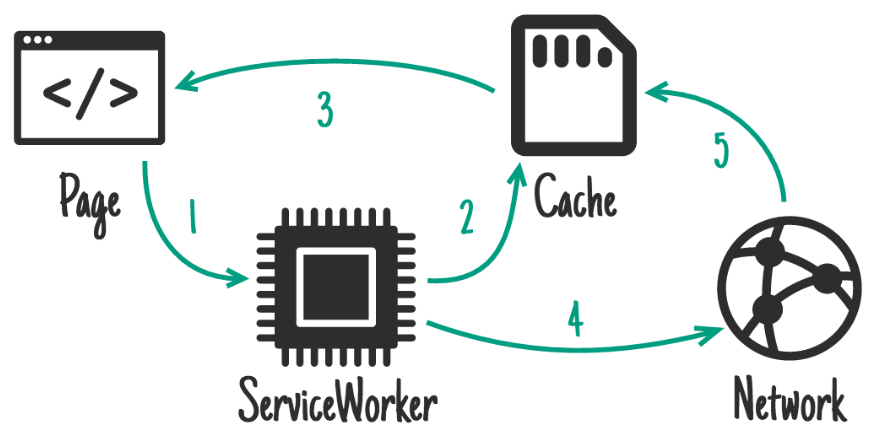
\includegraphics[width=200px]{ServiceWorker/StaleWhileRevalidate}\centering
	\caption{Voorstelling stale-while-revalidate strategie}
\end{figure}

\subsubsection{Offline first}
Bij deze strategie gaat de service worker kijken of de aangevraagde data al reeds gecached is op het apparaat. Als de data al reeds opgeslagen is op het apparaat, dan gebruikt de service worker de data die al reeds gecached is. Is er reeds geen data opgeslagen dan gaat de service worker via het netwerk de externe data opvragen. Eén van de grote nadelen van deze strategie is dat de externe data niet altijd up to date is.

\begin{figure}[!h]
	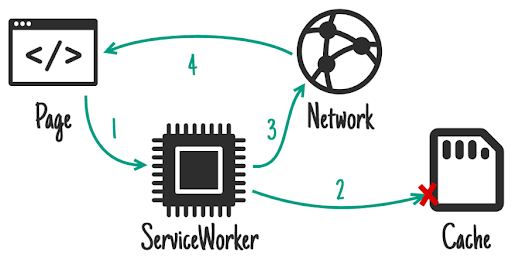
\includegraphics[width=200px]{ServiceWorker/OfflineFirst}\centering
	\caption{Voorstelling offline first strategie}
\end{figure}

\subsubsection{Online first}
Bij online first zal de service worker eerst de aanvraag doen via het netwerk. Als er geen netwerkverbinding is zal de service worker de gecachte data weergeven indien deze aanwezig is. Om deze reden moet er altijd een netwerkverbinding zijn om alle data binnen te halen voordat de applicatie offline de data kan weergeven. Met deze strategie is de externe data altijd up to date indien er een netwerkverbinding is.

\begin{figure}[!h]
	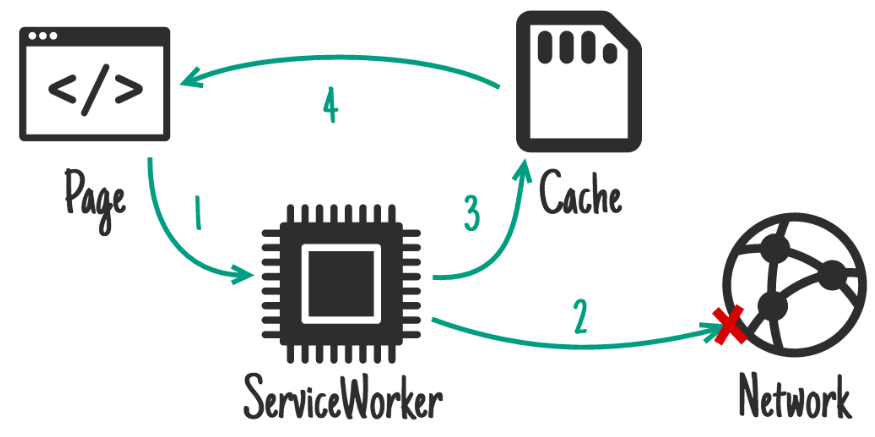
\includegraphics[width=200px]{ServiceWorker/OnlineFirst}\centering
	\caption{Voorstelling online first strategie}
\end{figure}

\subsubsection{Network Only}
Network only is een strategie die de externe data enkel maar via het netwerk zal ophalen. Als deze niet beschikbaar is zal de gecachte data ook niet weergegeven worden.

\begin{figure}[!h]
	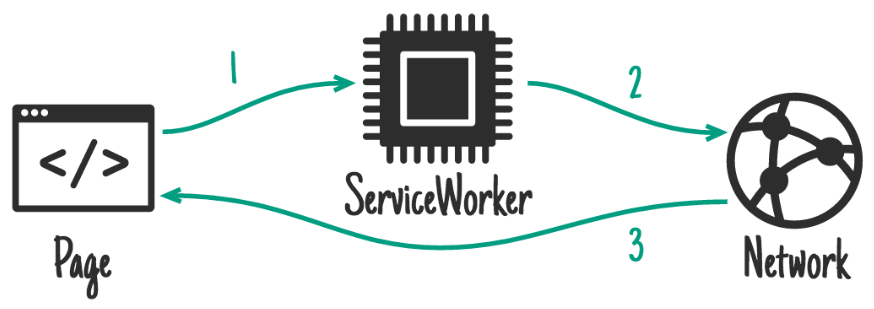
\includegraphics[width=200px]{ServiceWorker/NetworkOnly}\centering
	\caption{Voorstelling network only strategie}
\end{figure}

\subsubsection{Cache Only}
Cache only werkt alleen maar met de gecachte data. Deze haalt geen externe data gaan via het netwerk. Deze strategie kan gebruikt worden voor sites die geen externe data nodig hebben zoals een rekenmachine.

\begin{figure}[!h]
	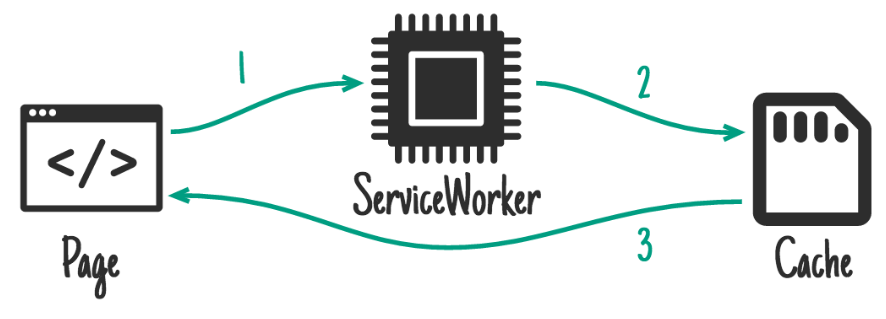
\includegraphics[width=200px]{ServiceWorker/CacheOnly}\centering
	\caption{Voorstelling cache only strategie}
\end{figure}

\subsection{Manifest}
Het tweede item dat een progressive web applicatie nodig heeft is een manifest (\cite{MANIFEST}). Dit is een bestand met alle informatie die nodig is om de applicatie draaiende te houden eens deze geïnstalleerd is op het apparaat. Deze informatie bevat maar is niet gelimiteerd tot de auteur, het icoon en de versie.

\subsubsection{Auteur}
De naam van de auteur van de applicatie. Deze kan ook de naam van het bedrijf zijn.

\subsubsection{Icoon}
Het icoon waarmee de applicatie wordt weergegeven bij de applicaties op het apparaat. Er kunnen verschillende iconen meegegeven worden. Deze kunnen dienen voor de verschillende besturingssystemen, zodat er bijvoorbeeld een uniek icoon is voor apple en android. De iconen kunnen ook een verschillende grootte hebben, dit zorgt ervoor dat het icoon goed zichtbaar is op elk scherm van de verscheidene apparaten.

\subsubsection{Versie}
De versie van applicatie wordt ingesteld worden door de manifest file. Zo weet de gebruiker welke versie van de applicatie er geïnstalleerd is op zijn apparaat.

\section{Frameworks}
\subsection{Wat is een framework ?}
Een Framework is een geheel van softwarecomponenten dat gebruikt kan worden bij het programmeren van applicaties. Ook de afspraken over hoe die componenten gebruikt worden binnen een groep ontwikkelaars en welke code-standaarden en bibliotheken gebruikt worden kunnen onderdeel zijn van een framework. Het framework bepaalt welke software er binnen een organisatie wordt gebruikt en op welke manier (\cite{WIKI_FRAMEWORK}).

\subsection{Requirements}
Wegens we de performance willen vergelijken tussen de twee frameworks zullen we gebruik maken van dezelfde backend applicatie namelijk google firebase.

De requirements voor de web applicatie zijn de volgende:

\begin{itemize}
	\item Service worker
	\item Manifest
	\item Router
	\item Store
	\item Data binding
\end{itemize}

De requirements voor de native applicatie zijn de volgende: 
\begin{itemize}
	\item Cross-platform
	\item Data binding
\end{itemize}

\subsection{Gekozen frameworks}
\subsubsection{Progressive web applicatie}
Er zijn verschillende frameworks voor een progressive web applicatie te ontwikkelen, maar op basis van bovenstaande requirement is er gekozen voor Vue.js in combinatie met Nuxt.js voor het creëren van de progressive web applicatie.
Andere mogelijkheden zijn (\cite{FRAMEWORKS_PROGRESSIVEWEBAPPS}) Angular, React, Ionic en Polymer.


\paragraph{Angular 2+}
Deze heeft ook een package om de site naar een progressive web applicatie te transformeren.
De reden waardoor angular niet geselecteerd werd, is omdat er een basiskennis van typescript aanwezig moet zijn voordat er een applicatie kan gebouwd worden. Anderzijds werd er beslist om met Vue te werken wegens dit het best beoordeelde framework is (\cite{VUE_POPULARITY}).

\paragraph{React}
React is geen officieel framework maar een library. Toch wordt deze opgenomen in de mogelijkheden omwille dat er een progressive web applicatie ontworpen kan worden met react. Deze werd niet geselecteerd omdat de programmeur een kennis van JSX hebben om react te kunnen gebruiken.

\paragraph{Ionic}
Ionic werd niet geselecteerd omwille dat de applicatie frequent moet geüpdatet worden om mee te kunnen met de laatste veranderingen van het framework (\cite{ICONIC}). Hierdoor kan de applicatie vrij snel verouderd worden. Als de site gebruik maakt van een verouderde package kan deze de site laten vastlopen.

\paragraph{Polymer}
De reden waarom polymer niet geselecteerd werd is dat het niet search engine optimised is (\cite{POLYMER}). Vervolgens heeft deze ook een hoge herlaadtijd voor de site.

\subsubsection{Native applicatie}
Om de native applicatie te ontwikkelen hebben is er gekozen voor het framework kotlin. Andere frameworks die in aanmerking kwamen waren Java en Xamarin.

\paragraph{Java}
Java is een populair framework onder de developers. Deze wordt nog altijd gebruikt voor allerhande applicaties, van bureaublad applicaties tot android applicaties. Kotlin heeft vele aspecten van java maar heeft deze beter gemaakt. Om die reden wordt de performantie hoger bij het gebruik van het Kotlin framework dan het Java framework. (\cite{KOTLIN_VS_JAVA})

\paragraph{Xamarin}
Xamarin werd niet geselecteerd door dat de performantie op het android platform niet optimaal is. De performantie op ios is veel beter. Bijkomend zijn er maar een paar ondersteunende Integrated development environments (IDE’s). Xamarin heeft ook geen ondersteuning voor android xml files die nodig zijn voor de opmaak. Om deze reden worden veel fouten gemaakt bij de xml bestanden tijdens de programmatie van de applicatie. (\cite{KOTIN_VS_XAMARIN}).


\subsection{Browserondersteuning}
Een browser moet een PWA kunnen ondersteunen voor deze uitgevoerd kan worden. Omwille dat de PWA functionaliteit nog maar vier jaar oud is is deze nog niet overal geïmplementeerd. Hieronder wordt bekeken of de bekendste browsers de PWA functionaliteit al ondersteunen. De ondersteuning van de PWA functionaliteit in Safari kon niet gevalideerd worden wegens dat er geen apparaat beschikbaar was met Safari.

\subsubsection{Chrome}
Wegens dat de PWA functionaliteit ontwikkeld is door Google is chrome de eerste browser die deze ondersteund. Chrome kan de PWA zowel op mobiel als op computer gebruiken. Eens deze applicatie geïnstalleerd is op mobiel zal deze verschijnen tussen de andere applicaties, op de computer zal deze verschijnen bij het tabblad chrome://apps.

\subsubsection{Firefox}
Firefox ondersteunt standaard de PWA functionaliteit niet op de computer. Deze kan wel aangezet worden door een paar instellingen te wijzigen.
Op mobiel ondersteunt Firefox de PWA functionaliteit wel met de Firefox Browser app, dit betekent dat de applicatie installeerbaar is. Na installatie is er een icoon te zien op het home scherm, maar niet in de applicaties zoals bij google chrome.

\subsubsection{Opera}
De PWA functionaliteit wordt helaas nog niet ondersteund op de computer. De service worker daarentegen wel. Deze zorgt ervoor dat de site nog beschikbaar is als het internet uitvalt. 
De mobiele versie van Opera (Opera Browser with free VPN) ondersteunt de PWA functionaliteit wel. Na installatie zal er net zoals bij de firefox browser een icoon te zien zijn op het home scherm maar zal deze niet voorkomen in de applicaties op het apparaat.
Verder werd er ook gekeken naar de nieuwe mobiele applicatie Opera Touch. Deze ondersteunt PWA functionaliteit niet.

\subsubsection{Safari}
Safari ondersteunt sinds IOS 11.3 de PWA functionaliteit. Na de installatie is de applicatie terug te vinden bij de andere applicaties op het home scherm. Aangezien de applicatie te installeren is via de browser heeft de applicatie geen quality test van apple ondergaan. Apple heeft een paar limitaties opgelegd aan deze soort applicaties zodat het apparaat nog altijd optimaal zou beschermd zijn. Een paar van deze limitaties zijn dat de applicatie maximaal 50 megabyte aan data mag verzamelen offline, er geen communicatie kan ontstaan tussen verschillende Apple-services zoals app betalingen en er geen push notifications ondersteund worden (\cite{BROWSERSUPPORT_IOS}).

\subsection{Store}
Deze sectie geeft een breder inzicht of de PWA site toegevoegd kan worden in de app store en play store.

\subsubsection{Play Store}
Google heeft reeds in 2019 beslist om de PWA functionaliteit toe te voegen aan de store (\cite{PLAYSTORE}). Voor een PWA in de play store te kunnen toevoegen moet er een native applicatie met de nodige certificaten worden aangemaakt met in de applicatie een verwijzing naar de PWA site. Op deze manier zal de applicatie de laatste data tonen van de PWA site zonder elke versie te moeten opladen naar de play store. Enkel voor grote veranderingen binnen de applicatie zoals het icoon, het manifest bestand, en de TWA(Trusted Web Activity) moet er een nieuwe versie geupload worden naar de play store.

\subsubsection{App Store}
Voor je een PWA kan uploaden in de app store heb je een native wrapper nodig zoals Cordova. Deze zet de code om naar een Xcode project, dit draagt het nadeel met zich mee dat een PWA enkel op een MacOs apparaat kan geüpload worden in de store. (\cite{APPSTORE})

\chapter{\IfLanguageName{dutch}{Kotlin}{Kotlin}}
\label{ch:kotlin}
Kotlin is een cross-platform programmeertaal, ontworpen om naadloos samen te werken met Java. Deze wordt officieel ondersteund door Google voor het ontwikkelen van mobiele apps op Android (\cite{KOTLIN}).

\section{\IfLanguageName{dutch}{Basisprincipes}{Basisprincipes}}
\label{sec:basisprincipes}

% NULL SAFETY
\subsection{Null safety}
%VARIABLE
Null saftey of null veiligheid is een feature die ingebouwd is in Kotlin (\cite{NULL_SAFETY}). Deze feature zorgt ervoor dat variabelen niet de waarde null kunnen bevatten. Als een variabele null zou kunnen bevatten geeft Kotlin hierop een error. Door deze feature kan je met Kotlin bijna nooit een null pointer error hebben. 

\begin{lstlisting}[caption=Null safty variablen, language=Kotlin]
var a: String = "abc"
a = null // error
\end{lstlisting}


%LIVEDATA
Dit is echter wel mogelijk als er een livedata variable of varianten hiervan worden aangemaakt. De livedata waarde List<String> wordt altijd geïnitieerd met null, indien dit niet gewenst is kan men deze altijd meegeven met een beginwaarde tussen de haakjes.

\begin{lstlisting}[caption=Null safty LiveData, language=Kotlin]
var c = MutableLiveData<List<String>>()
\end{lstlisting}


%NULL SAFTY OVERRIDE
Om de null veiligheid te overschrijven moet er een vraagteken geplaatst worden naast het datatype. Het vraagteken slaat erop dat de variabele nu de waarde null of een waarde van het datatype kan bevatten.

\begin{lstlisting}[caption=Overschrijf null safty, language=Kotlin]
var b: String? = "abc" // kan met null geïnstalleerd worden
b = null // ok
\end{lstlisting}


%NULL SAFTY OVERRIDE WARNING
Indien Kotlin een waarschuwing geeft bij een waarde die geen null kan zijn kunnen er twee uitroeptekens bij geplaatst worden Door dit te doen gaat kotlin ervanuit dat de waarde b nooit een null kan bevatten op die lijn code.

\begin{lstlisting}[caption=Waarschuwing null safty overschrijven, language=Kotlin]
val l = b!!.length
\end{lstlisting}


% LIVEDATA
\subsection{LiveData}
Livedata (\cite{LIVEDATA}) is een observable die lifecycle-aware is. Dit betekent dat livedata de lifecycle van de verschillende app componenten zoals activiteiten, fragmenten en services respecteert.

\begin{lstlisting}[caption=LiveData, language=Kotlin]
var c = MutableLiveData<List<String>>()
\end{lstlisting}


% LIFECYLE AWARE
Aangezien livedata lifecycle-aware is moet ervoor het observeren van de livedata variable geen rekening gehouden worden met de verschillende staten dat de applicatie in komt. Hieronder is er een voorbeeld zichtbaar van een observatie van een livedata variable c.

\begin{lstlisting}[caption=Observe liveData, language=Kotlin]
c.observe(viewLifecycleOwner, Observer {
	a = it
})
\end{lstlisting}


% Databinding
\subsection{Databinding}
Databinding (\cite{KOTLIN_DATABINDING}) zorgt ervoor dat de data in de UI automatisch wordt geüpdatet indien er een nieuwe waarde is van de variabele userName. Om deze te kunnen gebruiken moet er gebruik gemaakt worden van de layout tag, met hierin de data tag met welke variabele dat er moet gebind worden. Op deze manier wordt de scope van de data tag afgebakend. 

\begin{lstlisting}[caption=Databinding]
<layout xmlns:android="http://schemas.android.com/apk/res/android"
xmlns:app="http://schemas.android.com/apk/res-auto">

<data>
	<variable 
	name="viewmodel"
	type="com.myapp.data.ViewModel" />
</data>
<ConstraintLayout>
	<TextView android:text="@{viewmodel.userName}" />
</ConstraintLayout>
</layout>
\end{lstlisting}


% Coroutines
\subsection{Coroutines}
Coroutines (\cite{KOTLIN_COROUTINE}) zorgen ervoor dat er acties asynchroon worden uitgevoerd. Dit is nodig voor de main thread waar de applicatie op draait vrij te houden voor IO inputs zoals touch commands.
Zoals te zien is in onderstaand voorbeeld wordt er gebruik gemaakt van coroutines om een viewModelScope te lanceren. Alles binnen deze viewModelScope zal synchroon uitgevoerd worden op de applicatie.

\begin{lstlisting}[caption=Coroutine, language=Kotlin]
var c: List<String> = Arraylist<String>()

viewModelScope.launch {
	val repositoryResponse = async {
		repsitory.doSomething()
	}
	val dataOrError = repositoryResponse.await()
	if(dataOrError.hasError()){
		requestError.value = genericErrorMessage
	}else{
		c.clear()
		c.addAll(dataOrError.data)
	}
}
\end{lstlisting}

% Koin
\subsection{Koin}
Koin (\cite{KOTLIN_KOIN}) is een framework dat zorgt voor de dependency injection voor in een applicatie. Dependency injection is een ontwerppatroon om klassen te koppelen. Dit wil zeggen dat ze data kunnen uitwisselen zonder dat deze relatie vastgelegd is (\cite{KOTLIN_KOIN_DEPENDENCYINJECTION}).

\begin{lstlisting}[caption=Koin, language=Kotlin]
override fun onCreate() {
	super.onCreate()
	setupKoin()
	}

/**
* Setup DI with Koin.
*/
private fun setupKoin(){
	startKoin {
	androidLogger()
	androidContext(this@App)
	modules(listOf(repositoryModule))
}
}
/**
* Setup the repository module.
* Is public since we mock the repositories in tests.
*/
private val repositoryModule = module {
	single<IUserRepository> {
		UserRepository(get(), get(), get(),get(),get())
	}
}
\end{lstlisting}
\chapter{\IfLanguageName{dutch}{Vue.js}{Vue.js}}
\label{ch:vue}
Vue is een progressieve framework voor het bouwen van user interfaces. In tegenstelling tot andere monolithische kaders, wordt Vue vanaf de grond opgebouwd om stapsgewijs adoptable te zijn. De kernbibliotheek richt zich op de view layer alleen, en is gemakkelijk op te pikken en te integreren met andere bibliotheken of bestaande projecten. Aan de andere kant is Vue ook perfect in staat tot het voeden van geavanceerde Single-Page Applications bij gebruikt wordt in combinatie met moderne gereedschappen en ondersteunende bibliotheken (\cite{VUEJS}).

\section{\IfLanguageName{dutch}{Basisprincipes}{Basisprincipes}}
\label{sec:basisprincipes}

% Declarative Rendering
\subsection{Declarative Rendering}
Declarative Rendering (\cite{VUE_DECLARATIVERENDERING}) zorgt ervoor dat de data in de html automatisch word geüpdatet indien er een nieuwe waarde is van de variabele message. Dit komt omdat de data en de DOM gelinkt zijn met elkaar, hierdoor is alles reactief.

\begin{lstlisting}[caption=Declarative rendering html, language=HTML]
<div id="app">
	{{ message }}
</div>
\end{lstlisting}

\begin{lstlisting}[caption=Declarative rendering javascript, language=Javascript]
var app = new Vue({
	el: '#app',
	data: {
		message: 'Hello Vue!'
	}
})
\end{lstlisting}

We kunnen de data ook op een andere manier linken met een html component. Deze gebruikt de v-bind: tag met de naam van het attribuut erachter. Dit zorgt ervoor dat de span title gebind is aan de waarde van message.

\begin{lstlisting}[caption=Declarative rendering html alternatief, language=HTML]
<div id="app">
	<span v-bind:title="message">
		Test bericht
	</span>
</div>
\end{lstlisting}


%Conditionals
\subsection{Conditionals}
In vue is er een mogelijkheid om verschillende html tags niet te renderen. Deze zijn gekend als conditionals (\cite{VUE_CONDITIONALSANDLOOPS}). Een conditional kan toegevoegd worden door een v-if attribuut toe te voegen aan de html tag. Deze zal valideren of de gegeven html tag moet gerenderd worden. 

\begin{lstlisting}[caption=Conditionals html, language=HTML]
<div id="app-3">
	<span v-if="seen">Now you see me</span>
</div>
\end{lstlisting}


%Loops
\subsection{Loops}
Loops (\cite{VUE_CONDITIONALSANDLOOPS}) kunnen toegevoegd worden aan html tags zodat deze meerdere keren worden gerenderd. Deze kan gebruikt worden voor lijsten weer te geven zonder voor elk element in de lijst een html li tag aan te maken.

\begin{lstlisting}[caption=Loops html, language=HTML]
<div id="app-4">
	<ol>
		<li v-for="todo in todos">
			{{ todo.text }}
		</li>
	</ol>
</div>
\end{lstlisting}

\begin{lstlisting}[caption=Loops javascript, language=Javascript]
var app4 = new Vue({
	el: '#app-4',
	data: {
		todos: [
			{ text: 'Learn JavaScript' },
			{ text: 'Learn Vue' },
			{ text: 'Build something awesome' }
		]
	}
})
\end{lstlisting}


%Components
\subsection{Components}
In Vue.js kan je gebruik maken van verschillende components (\cite{VUE_COMPONENTS}). Een component is een klein gedeelte van de site, dit kan bijvoorbeeld een footer zijn. Het is de bedoeling dat de programmeur de site opdeelt in kleine componenten. Door dit te doen kunnen de verschillende componenten hergebruikt worden op verschillende pagina’s.

\begin{lstlisting}[caption=Components javascript, language=Javascript]
// Define a new component called button-counter
Vue.component('button-counter', {
	data: function () {
		return {
			count: 0
		}
	},
	template: '<button v-on:click="count++">You clicked me {{ count }} times.</button>'
})
\end{lstlisting}

\begin{lstlisting}[caption=Components html, language=HTML]
<div id="components-demo">
	<button-counter></button-counter>
	<button-counter></button-counter>
	<button-counter></button-counter>
</div>
\end{lstlisting}
\chapter{\IfLanguageName{dutch}{Nuxt.js}{Nuxt.js}}
\label{ch:nuxt}
Nuxt.js is een framework voor vue.js applicaties met als doel om vue developers eerste klasse technologieën te laten implementeren zoals server side rendering (SSR), code splitting en pre rendering (\cite{NUXTJS}). Nuxt heeft ook een ingewerkte PWA library. Deze kan gebruikt worden om een site in een PWA te veranderen. 

\section{\IfLanguageName{dutch}{Basisprincipes}{Basisprincipes}}
\label{sec:basisprincipes}

% Server side rendering
\subsection{Server side rendering}
Server side rendering (\cite{NUXT_SERVERSIDERENDERING}) wordt gebruikt om je applicatie te renderen naar statische html en css bestanden. Na het doorsturen van de belangrijkste html en css bestanden worden deze weergegeven op het apparaat. Vervolgens zal de javascript bundel doorgestuurd worden. Dit betekend dat het apparaat geen gebruik kan maken van de javascript functionaliteit zolang deze bundel nog niet gedownload is. Pas na de parsing en uitvoering van de javascript bestand(en) op het apparaat kan hiervan gebruik gemaakt worden.

%Pre rendering
\subsection{Pre rendering}
Pre rendering (\cite{NUXT_PRERENDERING}) is gelijkaardig aan server side rendering. Het grootste verschil is dat pre rendering de pagina zal renderen en deze al opslaan als statisch bestand. Als deze dan wordt opgevraagd door het apparaat zal dit bestand niet nog eens gerenderd worden maar zal de een statische pagina teruggestuurd worden.

%Configuration
\subsection{Configuration}
Het configuration of configuratie (\cite{NUXT_CONFIGURATION}) bestand (nuxt.config.js) is waar alle instellingen van Nuxt geconfigureerd worden.

\begin{lstlisting}[caption=Configuration, language=Javascript]
export default {
	mode: 'universal',
/*
** Headers of the page
*/
	head: {
	title: process.env.npm_package_name || '',
	meta: [
		{ charset: 'utf-8' },
		{ name: 'viewport', content: 'width=device-width, initial-scale=1' },
		{ hid: 'description', name: 'description', content: process.env.npm_package_description || '' }
	],
	link: [
		{ rel: 'icon', type: 'image/png', href: '/icon.png' }
	]
	},
/*
** Customize the progress-bar color
*/
	loading: { color: '#fff' },
/*
** Global CSS
*/
	css: [],
/*
** Plugins to load before mounting the App
*/
	plugins: [],
/*
** Nuxt.js dev-modules
*/
	buildModules: [],
/*
** Nuxt.js modules
*/
	modules: [],
/*
** Build configuration
*/
	build: {
/*
** You can extend webpack config here
*/
		extend (config, ctx) {
		}
	}
}
\end{lstlisting}


%Directory Structure
\subsection{Directory Structure}
Standaard heeft Nuxt.js al een mappen structuur (\cite{NUXT_DIRECTORYSTRUCTURE}). Deze mappenstructuur is een goed beginpunt voor verschillende applicaties om een overzicht binnenin het project te bewaren. Indien de gebruiker deze structuur niet wilt gebruiken is deze vrij om de mappenstructuur aan te passen.

\begin{figure}[!h]
	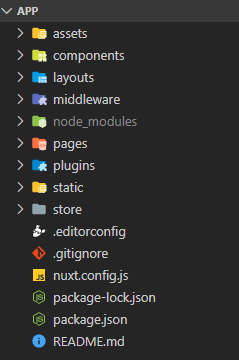
\includegraphics[width=200px]{Nuxt/Nuxt_DirectoryStructure}\centering
	\caption{Voorbeeld mappen structuur nuxt}
\end{figure}


%Routing
\subsection{Routing}
Nuxt.js maakt het heel gemakkelijk om de verschillende routes (\cite{NUXT_ROUTING}) in de site te configureren. Het enige dat de gebruiker hoeft te doen is een map genereren met de naam van de route en een index.vue bestand aanmaken waar nuxt standaard naartoe zal navigeren indien er geen parameters aan te pas komen.

\begin{lstlisting}[caption=Routering mappenstuctuur]
pages/
--| user/
-----| index.vue
-----| one.vue
--| index.vue
\end{lstlisting}

Bovenstaande mappenstructuur zal deze routes genereren:

\begin{lstlisting}[caption=Routering generatie]
router: {
	routes: [
		{
			name: 'index',
			path: '/',
			component: 'pages/index.vue'
		},
		
		{
			name: 'user',
			path: '/user',
			component: 'pages/user/index.vue'
		},
		
		{
			name: 'user-one',
			path: '/user/one',
			component: 'pages/user/one.vue'
		}
	]
}
\end{lstlisting}

Indien er parameters aan te pas komen moet de gebruiker in plaats van een index.vue te creëren een bestand maken met als naam ‘\_ naam van de parameter’. Hierdoor wordt naar deze pagina genavigeerd indien die parameter aanwezig is.

\begin{lstlisting}[caption=Routering mappenstructuur met id parameter]
pages/
--| users/
-----| _id.vue
--| index.vue
\end{lstlisting}

Bovenstaande mappenstructuur zal onderstaande routes genereren: 

\begin{lstlisting}[caption=Routering generatie met id parameter]
router: {
	routes: [
		{
			name: 'index',
			path: '/',
			component: 'pages/index.vue'
		},
		{
			name: 'users-id',
			path: '/users/:id?',
			component: 'pages/users/_id.vue'
		}
	]
}
\end{lstlisting}


%Vuex Store
\subsection{Vuex Store}
Vuex Store (\cite{NUXT_VUEXSTORE}) wordt standaard met Nuxt.js meegeleverd. Dit wordt gebruikt om verschillende gegevens te beheren. De Vuex store wordt opgebouwd uit verschillende modules, tijdens het bouwen van de website worden deze modules samengevoegd en geconfigureerd als Vuex store.

\begin{lstlisting}[caption=Vuex store index.js, language=Javascript]
export const state = () => ({
	counter: 0
})

export const mutations = {
	increment (state) {
		state.counter++
	}
}
\end{lstlisting}

\begin{lstlisting}[caption=Vuex store todos.js, language=Javascript]
export const state = () => ({
	list: []
})

export const mutations = {
	add (state, text) {
		state.list.push({
			text,
			done: false
		})
	},
	remove (state, { todo }) {
		state.list.splice(state.list.indexOf(todo), 1)
	},
	toggle (state, todo) {
		todo.done = !todo.done
	}
}
\end{lstlisting}

Bovenstaande bestanden worden geconfigureerd als volgend vuex store:

\begin{lstlisting}[caption=Vuex store, language=Javascript]
new Vuex.Store({
	state: () => ({
		counter: 0
	}),
	mutations: {
		increment (state) {
			state.counter++
		}
	},
	modules: {
		todos: {
			namespaced: true,
			state: () => ({
				list: []
			}),
			mutations: {
				add (state, { text }) {
					state.list.push({
						text,
						done: false
				})
			},
			remove (state, { todo }) {
				state.list.splice(state.list.indexOf(todo), 1)
			},
			toggle (state, { todo }) {
				todo.done = !todo.done
			}
		}
	}
})
\end{lstlisting}

Een andere mogelijkheid om de store op te bouwen is om de modules over verschillende bestanden te spreiden. In de store map staan er dan vier bestanden: state.js, actions.js, mutations.js en getters.js.


%Modules
\subsection{Modules}
Modules (\cite{NUXT_MODULES}) zijn Nuxt.js extensies waarmee de Nuxt functionaliteit uitgebreid kan worden met de volgende functionaliteiten: @nuxt/http, @nuxt/axios, @nuxt/pwa en @nuxt/auth. Deze modules kunnen verder uitgebreid worden met eigen geschreven modules.

\subsubsection{@nuxt/http}
Dit is een universele manier om HTTP-aanvragen te doen.

\subsubsection{@nuxt/axios}
De nuxt axios module gebruikt het axios pakket om HTTP-aanvragen te doen.

\subsubsection{@nuxt/pwa}
De pwa module zorgt ervoor dat je applicatie een progressive web app wordt. Dit zorgt ervoor dat de webapplicatie geïnstalleerd kan worden als een native applicatie op het apparaat.

\subsubsection{@nuxt/auth}
Deze module zorgt voor de authenticatie van de gebruikers.


%Plugins
\subsection{Plugins}
Plugins (\cite{NUXT_PLUGINS}) worden gebruikt om externe pakketten toe te voegen aan de applicatie. In de plugin wordt de configuratie van het gekozen pakket gedefinieerd. Na het configureren van de plugin moet deze toegevoegd worden aan de plugins in het configuratiebestand van Nuxt. In onderstaand voorbeeld wordt Vue material geconfigureerd.

\begin{lstlisting}[caption=Vue material plugin, language=Javascript]
import Vue from 'vue'
import VueMaterial from 'vue-material'
import 'vue-material/dist/vue-material.min.css'
import '~/assets/scss/material.scss' // css presets

Vue.use(VueMaterial)
\end{lstlisting}

Toe te voegen aan nuxt.config.js:

\begin{lstlisting}[caption= Plugin toevoegen aan nuxt.config.js, language=Javascript]
plugins: ['~/plugins/vue-notifications']
\end{lstlisting}

Indien de plugin een ES6 module exporteert moet deze ook toegevoegd worden aan de transpile optie binnen in het configuratiebestand.

\begin{lstlisting}[caption= Plugin toevoegen aan nuxt.config.js transpile, language=Javascript]
build: {
	transpile: ['vue-notifications']
}
\end{lstlisting}
%%=============================================================================
%% Methodologie
%%=============================================================================

\chapter{\IfLanguageName{dutch}{Methodologie}{Methodology}}
\label{ch:methodologie}

%% TODO: Hoe ben je te werk gegaan? Verdeel je onderzoek in grote fasen, en
%% licht in elke fase toe welke stappen je gevolgd hebt. Verantwoord waarom je
%% op deze manier te werk gegaan bent. Je moet kunnen aantonen dat je de best
%% mogelijke manier toegepast hebt om een antwoord te vinden op de
%% onderzoeksvraag.

\section{Performantie vergelijking}
\subsubsection{Gebruikte software}
Progressive web applicatie

Native applicatie

\subsubsection{Apparaten}
Progressive web applicatie

Native applicatie

\subsubsection{Vergelijking}

FILTERTEST
\begin{table}[]
	\begin{tabular}{cccccc}
		Type        & Min.  & 1ste Qu. & Gemiddelde & 3de Qu. & Max.  \\
		PWA         & 2.380 & 2.522    & 2.693      & 2.745   & 4.360 \\
		Offline PWA & 2.460 & 2.565    & 2.752      & 2.992   & 3.350 \\
		Native App  & 2.118 & 2.152    & 2.360      & 2.474   & 2.950 
	\end{tabular}
\end{table}



DETAIL MENU TEST
\begin{table}[]
	\begin{tabular}{cccccc}
		Type        & Min.  & 1ste Qu. & Gemiddelde & 3de Qu. & Max.  \\
		PWA         & 2.940 & 3.205    & 3.380      & 3.465   & 4.170 \\
		Offline PWA & 2.050 & 3.138    & 3.292      & 3.478   & 4.610 \\
		Native App  & 2.596 & 2.826    & 2.846      & 2.901   & 2.952
	\end{tabular}
\end{table}



% Voeg hier je eigen hoofdstukken toe die de ``corpus'' van je bachelorproef
% vormen. De structuur en titels hangen af van je eigen onderzoek. Je kan bv.
% elke fase in je onderzoek in een apart hoofdstuk bespreken.

%\input{...}
%\input{...}
%...

%%=============================================================================
%% Conclusie
%%=============================================================================

\chapter{Conclusie}
\label{ch:conclusie}

% TODO: Trek een duidelijke conclusie, in de vorm van een antwoord op de
% onderzoeksvra(a)g(en). Wat was jouw bijdrage aan het onderzoeksdomein en
% hoe biedt dit meerwaarde aan het vakgebied/doelgroep? 
% Reflecteer kritisch over het resultaat. In Engelse teksten wordt deze sectie
% ``Discussion'' genoemd. Had je deze uitkomst verwacht? Zijn er zaken die nog
% niet duidelijk zijn?
% Heeft het onderzoek geleid tot nieuwe vragen die uitnodigen tot verder 
%onderzoek?




%%=============================================================================
%% Bijlagen
%%=============================================================================

\appendix
\renewcommand{\chaptername}{Appendix}

%%---------- Onderzoeksvoorstel -----------------------------------------------

\chapter{Onderzoeksvoorstel}

Het onderwerp van deze bachelorproef is gebaseerd op een onderzoeksvoorstel dat vooraf werd beoordeeld door de promotor. Dat voorstel is opgenomen in deze bijlage.

% Verwijzing naar het bestand met de inhoud van het onderzoeksvoorstel
\graphicspath{ {./Img/} }

%---------- Inleiding ---------------------------------------------------------

\section{Introductie} % The \section*{} command stops section numbering
\label{sec:introductie}
De native app kende de afgelopen jaren een enorme groei in aantal gebruikers en werd de voornaamste manier om apps te maken. Er was oorspronkelijk wel een groot nadeel, namelijk dat de app apart moest worden geprogrammeerd voor android en voor ios. Hierdoor waren er verschillende code bases waardoor het onderhoud van de app moeilijker werd. Dit werd later opgelost door cross-platform development. Het nadeel hiervan is dat de categorieën zich vandaag niet meer beperken tot smartphone en tablets. Daarnaast blijft de app ook kampen met onderhoudsproblemen, vanwege bepaalde features die enkel beschikbaar zijn op ios. Aldus werd er verder gezocht naar een oplossing. Die is er nu, namelijk de progressive web app (PWA). Dit is een app die je gemakkelijk kan installeren op zowel android als op ios. Hierdoor los je het probleem op van de native apps. Namelijk dat een PWA maar 1 code base heeft voor alle platformen(\cite{Why_PWA_over_NativeApp}).
% onderzoeksvragen
Deze bachlorproef beseert zich op de volgende onderzoeksvragen.
\begin{itemize}
	\item Wat zijn de voordelen van PWA vs Cross-Platform Native Apps?
	\item Welke frameworks komen hiervoor in aanmerking?
	\item Wat is de impact op de gebruikerservaring en toegankelijkheid ?
	\item Zal de PWA de native app vervangen?
	
\end{itemize}

%Intro
%Hier introduceer je werk. Je hoeft hier nog niet te technisch te gaan.

%Je beschrijft zeker:

%\begin{itemize}
%  \item de probleemstelling en context
%  \item de motivatie en relevantie voor het onderzoek
%  \item de doelstelling en onderzoeksvraag/-vragen
%Mobiele applicatieontwikkeling\end{itemize}

%---------- Stand van zaken ---------------------------------------------------

\section{Stand van zaken}
\label{sec:stand van zaken}
Er zijn reeds onderzoeken uitgevoerd die de verschillende
voor- en nadelen van een PWA en van een Cross-Platform app met elkaar vergelijken. Aldus onderzoekt men de mogelijkheid om native apps te vervangen door progressive web apps.
Deze onderzoeken staan beschreven in artikels zoals die van \cite{PWA_vs_Cross-Platform}, \cite{Tinder_PWA} en \cite{Webview_PWA}

Uit onderzoek van \cite{Tinder_PWA} blijkt dat een PWA de performantie toch wel kan verhogen in vergelijking met een native app. Dit omdat de ruimte voor de app te installeren veel kleiner is dan een native app. Daarentegen vond ik terug in artikel \cite{PWA_vs_Cross-Platform} dat er nog geen zekerheid is of een native app kan vervangen worden door een PWA.
Daarnaast stelt Marjchzak dat PWA’s nog niet supported zijn binnen het apple ecosysteem. Dit omdat safari nog geen ondersteuning biedt om een service worker te draaien op het systeem. Aangezien een service worker ervoor zorgt dat een PWA alle data cached, is deze essentieel voor het bouwen van een progressive web application. Als deze data terug moet opgehaald worden als er geen internet verbinding is, haalt hij deze van de service worker die het op zijn beurt ophaalt van de cash van het systeem. Hierdoor kan de PWA offline blijven werken eens alle data geladen is.



%Hier beschrijf je de \emph{state-of-the-art} rondom je gekozen onderzoeksdomein. Dit kan bijvoorbeeld een literatuurstudie zijn. Je mag de titel van deze sectie ook aanpassen (literatuurstudie, stand van zaken, enz.). Zijn er al gelijkaardige onderzoeken gevoerd? Wat concluderen ze? Wat is het verschil met jouw onderzoek? Wat is de relevantie met jouw onderzoek?

%Verwijs bij elke introductie van een term of bewering over het domein naar de vakliteratuur, bijvoorbeeld~\autocite{Doll1954}! Denk zeker goed na welke werken je refereert en waarom.

% Voor literatuurverwijzingen zijn er twee belangrijke commando's:
% \autocite{KEY} => (Auteur, jaartal) Gebruik dit als de naam van de auteur
%   geen onderdeel is van de zin.
% \textcite{KEY} => Auteur (jaartal)  Gebruik dit als de auteursnaam wel een
%   functie heeft in de zin (bv. ``Uit onderzoek door Doll & Hill (1954) bleek
%   ...'')

%Je mag gerust gebruik maken van subsecties in dit onderdeel.

%---------- Methodologie ------------------------------------------------------
\section{Methodologie}
\label{sec:methodologie}
Om de performantie van de verschillende apps te vergelijken zal er twee maal eenzelfde applicatie gebouwd worden. Op android wordt deze gemaakt met framework kotlin, de PWA zal gemaakt worden met behulp van het framework vue.js in combinatie met nuxt. Op deze apps zullen verschillende soorten operaties uitgevoerd kunnen worden. Elk van deze operaties zal meermaals worden uitgevoerd en ondertussen zal de snelheid getest worden. Deze verkregen resultaten zullen vervolgens met elkaar vergeleken worden om te bepalen welke applicatie het meest performant is. Naast het onderzoek naar de performantie zal er ook onderzoek worden gedaan naar hoeveel ruimte deze app inneemt op een apparaat. Ook deze resultaten zullen worden vergeleken.

%Hier beschrijf je hoe je van plan bent het onderzoek te voeren. Welke onderzoekstechniek ga je toepassen om elk van je onderzoeksvragen te beantwoorden? Gebruik je hiervoor experimenten, vragenlijsten, simulaties? Je beschrijft ook al welke tools je denkt hiervoor te gebruiken of te ontwikkelen.

%---------- Verwachte resultaten ----------------------------------------------
\section{Verwachte resultaten}
\label{sec:verwachte_resultaten}
Om de resultaten voor te stellen wordt er gebruik gemaakt van een boxplot, zoals te zien is op figuur 1. Er zal er ook nog een tabel komen die de boxplot weergeeft. De getallen die hierin terug te vinden zijn: het gemiddelde, het maximum, het minimum, eerste kwadrant en derde kwadrant. Hierdoor krijgen we een goed overzicht om de resultaten te vergelijken tussen de PWA en native app.

\begin{figure}[!h]
	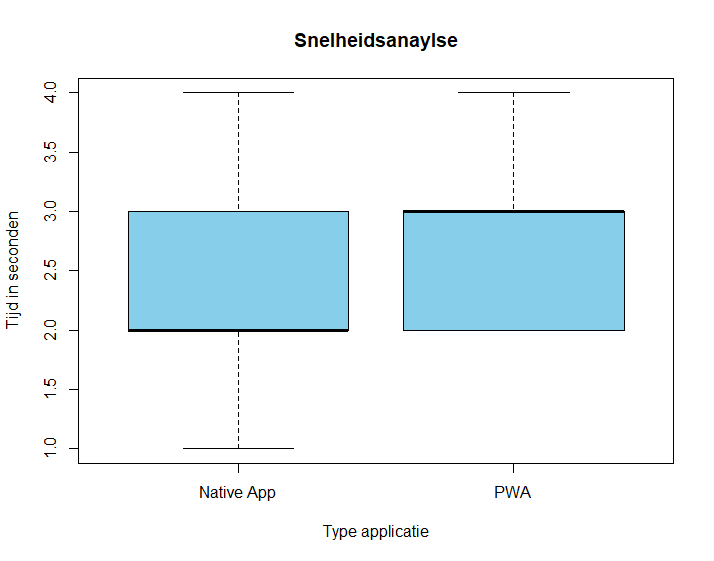
\includegraphics[width=200px]{Rplot_Boxplot_Snelheidsanalyse.png}\centering
	\caption{Voorbeeld van boxplot die de snelheid vergelijkt}
\end{figure}

\begin{figure}[!h]
	\begin{tabularx}{\textwidth /2 }{|X|X|X|X|X|X|}
		\hline
		 & min. & 1ste kwadrant & Gem. & 3de kwadrant & max. \\
		\hline
		PWA & 2 & 2 & 2.714 & 3 & 4 \\
		\hline
		native app & 1 & 1 & 2.429 & 3 & 4 \\
		\hline
	\end{tabularx}
	\caption{Voorbeeld van een tabel die de snelheid vergelijkt}
\end{figure}


Voor de resultaten van de benodigde ruimte weer te geven zal gebruik gemaakt worden van een historiek, zoals te zien is op figuur 3. Er zal zoals bij de vergelijking van de tijd ook een tabel zijn met alle info die de historiek weergeeft.

\begin{figure}[!h]
	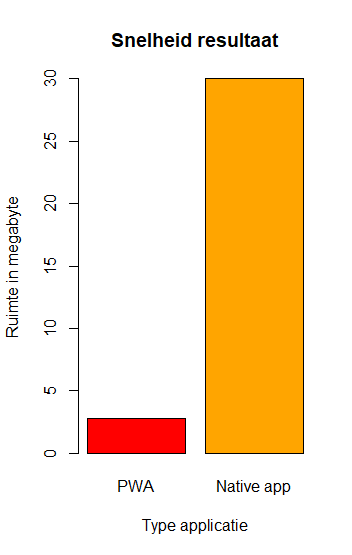
\includegraphics[width=120px]{Rplot_Ruimte_PWAvsNativeApp.png}\centering
	\caption{Voorbeeld van historgram die de benodigde ruimte vergelijkt}
\end{figure}


% tabel benodigde ruimte
\begin{figure}[!h]
\begin{tabular}{ |p{10em}|c|c| }
	\hline
	Type applicatie & Benodigde ruimte \\
	\hline
	progressive web app & 2.8 MB \\
	\hline
	native app & 30 \\
	\hline
\end{tabular}
\caption{Voorbeel van tabel die de benodigde ruimte vergelijkt}
\end{figure}


%Hier beschrijf je welke resultaten je verwacht. Als je metingen en simulaties uitvoert, kan je hier al mock-ups maken van de grafieken samen met de verwachte conclusies. Benoem zeker al je assen en de stukken van de grafiek die je gaat gebruiken. Dit zorgt ervoor dat je concreet weet hoe je je data gaat moeten structureren.

%---------- Verwachte conclusies ----------------------------------------------
\section{Verwachte conclusies}
\label{sec:verwachte_conclusies}
Er wordt verwacht dat de snelheid niet significant verschillend zal zijn tussen de PWA en de native app. De native app haalt enkel de content op waardoor deze net iets sneller zal zijn. De PWA moet alle data ophalen samen met de layout , dit is de data moet weergegeven worden. Hierdoor zal de PWA een x tal milliseconden trager zijn dan de native applicatie

Verder wordt er verwacht dat de benodigde ruimte op een apparaat significant minder zal zijn dan de native app. Dit komt doordat de native app op het apparaat zelf geïnstalleerd is. Hierdoor staat er een standaard layout geïnstalleerd op het apparaat, wat redelijk veel ruimte inneemt. De PWA haalt zowel zijn inhoud als zijn layout van een server. Hierdoor kan een PWA de benodigde ruimte op het apparaat beperken. 

%Hier beschrijf je wat je verwacht uit je onderzoek, met de motivatie waarom. Het is \textbf{niet} erg indien uit je onderzoek andere resultaten en conclusies vloeien dan dat je hier beschrijft: het is dan juist interessant om te onderzoeken waarom jouw hypothesen niet overeenkomen met de resultaten.



%%---------- Andere bijlagen --------------------------------------------------
% TODO: Voeg hier eventuele andere bijlagen toe
%\input{...}

%%---------- Referentielijst --------------------------------------------------

\printbibliography[heading=bibintoc]

\end{document}
